\documentclass{article}
\usepackage{amsmath}
\usepackage{tikz}
\usetikzlibrary{matrix, arrows.meta}

\begin{document}

\section*{Two Permutations $\sigma_0, \sigma_1$ on Twelve Solutions $\Omega_{\mathbf{u}}$}

In the middle, $\sigma_0$ is written in cycle notation, whereas $\sigma_1$ is represented via arrows. A solid arrow from a boxed founder indicates an instance of line \texttt{6} in Algorithm \ref{alg:monodromy_solve} proceeding to line \texttt{8}.

\begin{figure}[h]
    \centering
    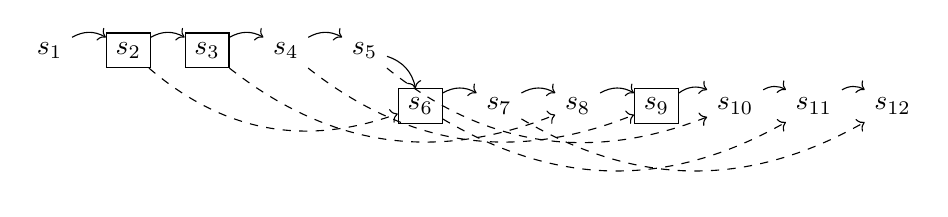
\begin{tikzpicture}[node distance=1cm, auto]
        % Define nodes
        \node (s1) {$s_1$};
        \node[draw, rectangle, right of=s1] (s2) {$s_2$};
        \node[draw, rectangle, right of=s2] (s3) {$s_3$};
        \node[right of=s3] (s4) {$s_4$};
        \node[right of=s4] (s5) {$s_5$};
        \node[draw, rectangle, below right of=s5] (s6) {$s_6$};
        \node[right of=s6] (s7) {$s_7$};
        \node[right of=s7] (s8) {$s_8$};
        \node[draw, rectangle, right of=s8] (s9) {$s_9$};
        \node[right of=s9] (s10) {$s_{10}$};
        \node[right of=s10] (s11) {$s_{11}$};
        \node[right of=s11] (s12) {$s_{12}$};

        % Draw arrows for sigma_0
        \draw[->] (s1) to[bend left] (s2);
        \draw[->] (s2) to[bend left] (s3);
        \draw[->] (s3) to[bend left] (s4);
        \draw[->] (s4) to[bend left] (s5);
        \draw[->] (s5) to[bend left] (s6);
        \draw[->] (s6) to[bend left] (s7);
        \draw[->] (s7) to[bend left] (s8);
        \draw[->] (s8) to[bend left] (s9);
        \draw[->] (s9) to[bend left] (s10);
        \draw[->] (s10) to[bend left] (s11);
        \draw[->] (s11) to[bend left] (s12);

        % Draw dashed arrows for sigma_1
        \draw[dashed, ->] (s2) to[bend right] (s6);
        \draw[dashed, ->] (s3) to[bend right] (s8);
        \draw[dashed, ->] (s4) to[bend right] (s9);
        \draw[dashed, ->] (s5) to[bend right] (s10);
        \draw[dashed, ->] (s6) to[bend right] (s11);
        \draw[dashed, ->] (s7) to[bend right] (s12);
    \end{tikzpicture}
\end{figure}

\end{document}